% Reader's companion to the cutoff-removal theorem -- SCAFFOLD (R0, 23 October 2026).
% Everything below the preamble is placeholder structure for the toolchain test; the
% editor's PLAN.md (round R2) replaces it.  Build: pdflatex x3 from this folder.
\documentclass[11pt,a4paper]{article}
% Preamble of the reader's companion.  Shared with the figure test builds.
\usepackage[margin=30mm]{geometry}
\usepackage[T1]{fontenc}
\usepackage{amsmath,amssymb,amsthm,mathtools,mathrsfs}
\usepackage{microtype,booktabs,enumitem,longtable,array}
\usepackage{xcolor}
% Colours: the documentation site's palette (docs/figures/svg.py, LIGHT), so that
% "conditional on U_GJS" is the same violet in the README, on the site and here.
\definecolor{noteBlue}{RGB}{30,72,110}
\definecolor{acc}{RGB}{9,105,218}     % #0969da  primary series / emphasis
\definecolor{warn}{RGB}{188,76,0}     % #bc4c00  second series / caution
\definecolor{cond}{RGB}{130,80,223}   % #8250df  conditional on U_GJS -- reserved
\definecolor{ok}{RGB}{26,127,55}      % #1a7f37  unconditional / closed
\definecolor{mut}{RGB}{110,119,129}   % #6e7781  muted ink, guides
\definecolor{gline}{RGB}{208,215,222} % #d0d7de  grid and frames
\definecolor{cfill}{RGB}{243,238,252} % #f3eefc  conditional fill
\definecolor{afill}{RGB}{221,244,255} % #ddf4ff  accent fill
\usepackage{tikz}
\usetikzlibrary{arrows.meta,positioning,calc,fit,backgrounds,decorations.pathreplacing,patterns}
\usepackage{pgfplots}
\pgfplotsset{compat=1.18}
\usepackage{fancyhdr}
\usepackage[colorlinks=true,linkcolor=noteBlue,citecolor=noteBlue,urlcolor=noteBlue]{hyperref}
\usepackage[most]{tcolorbox}

% Floats: let a tall figure share a page with text instead of waiting for a float page.
\renewcommand{\topfraction}{0.92}\renewcommand{\bottomfraction}{0.6}
\renewcommand{\textfraction}{0.06}\renewcommand{\floatpagefraction}{0.85}
\setcounter{topnumber}{2}\setcounter{totalnumber}{3}
\pagestyle{fancy}\fancyhf{}
\lhead{\small Reader's companion: cutoff removal for weakly coupled $P(\varphi)_2$}
\rhead{\small\thepage}
\renewcommand{\headrulewidth}{0.3pt}

% ---- the record's own macros, verbatim from part_i/main.tex lines 21-47 ----
\theoremstyle{plain}
\newtheorem{theorem}{Theorem}[section]
\newtheorem{proposition}[theorem]{Proposition}
\newtheorem{lemma}[theorem]{Lemma}
\newtheorem{corollary}[theorem]{Corollary}
\theoremstyle{definition}
\newtheorem{definition}[theorem]{Definition}
\newtheorem{remark}[theorem]{Remark}
\newtheorem{idea}{Idea}
\newcommand{\R}{\mathbb{R}}
\newcommand{\Z}{\mathbb{Z}}
\newcommand{\C}{\mathbb{C}}
\newcommand{\E}{\mathbb{E}}
\newcommand{\A}{\mathfrak{A}}
\newcommand{\G}{\mathcal{G}}
\newcommand{\CE}{\mathcal{C}_{\mathrm E}}
\newcommand{\CH}{\mathcal{C}_{\mathrm H}}
\newcommand{\HH}{\mathcal{H}}
\newcommand{\Om}{\Omega}
\newcommand{\ip}[2]{\langle #1,#2\rangle}
\DeclareMathOperator{\supp}{supp}
\DeclareMathOperator{\dist}{dist}
\DeclareMathOperator{\spec}{spec}
\DeclareMathOperator{\Span}{span}
\DeclareMathOperator{\Ran}{Ran}

% ---- companion-specific ----
% A locator into the document of record [R]: \rec{Theorem~12.2}{30}.
\DeclareRobustCommand{\rec}[2]{[\hyperlink{bib-record}{R}, #1, p.\,#2]}
\DeclareRobustCommand{\recpp}[2]{[\hyperlink{bib-record}{R}, #1, pp.\,#2]}
\newcommand{\UGJS}{U_{\mathrm{GJS}}}
\newcommand{\condtext}[1]{\textcolor{cond}{#1}}
% Boxes.  recordbox: a statement quoted from the record.  checkpoint: the displayed
% statement a reader holds on to at the end of a short chain.  statusnotice: page 1.
\newtcolorbox{recordbox}[1]{enhanced,breakable,colback=white,colframe=gline,
  coltitle=black,colbacktitle=gline!40!white,fonttitle=\bfseries\small,title={#1},
  boxrule=0.5pt,arc=1pt,left=6pt,right=6pt,top=4pt,bottom=4pt}
\newtcolorbox{checkpoint}[1][Checkpoint]{enhanced,colback=afill!60!white,colframe=acc,
  coltitle=white,colbacktitle=acc,fonttitle=\bfseries\small,title={#1},
  boxrule=0.5pt,arc=1pt,left=6pt,right=6pt,top=4pt,bottom=4pt}
\newtcolorbox{statusnotice}{enhanced,colback=warn!6!white,colframe=warn,
  boxrule=0.6pt,arc=1pt,left=6pt,right=6pt,top=4pt,bottom=4pt}
\newenvironment{context}{\par\noindent\textsc{Context, not part of the record.}\ }{\par}

% pgfplots house style: recessive grid, thin marks, text in ink colours.
\pgfplotsset{companion/.style={width=0.48\textwidth,height=0.36\textwidth,
  axis line style={gline},tick style={gline},grid=major,grid style={gline!60!white},
  tick label style={font=\scriptsize,color=mut},label style={font=\small},
  every axis plot/.append style={line width=0.9pt},
  legend style={font=\scriptsize,draw=none,fill=none},legend cell align=left}}



\title{A reader's companion to the cutoff-removal theorem\\[4pt]
  \large (scaffold: structure and toolchain test only)}
\author{Alexander Stottmeister\\[3pt]
  \normalsize Institut f\"ur Theoretische Physik, Leibniz Universit\"at Hannover,\\
  \normalsize Appelstra\ss e 2, 30167 Hannover, Germany}
\date{Draft of 23 October 2026}

\begin{document}
\maketitle

\begin{statusnotice}
\textbf{Status notice (placeholder; the editor's wording replaces it).} The result this
companion explains, Theorem~12.2 of the record \rec{Theorem~12.2}{30}, is proved
\condtext{conditional on $\UGJS$}, one imported hypothesis. Nothing in the record has been
refereed; audit item C5 is open; the record is AI-assisted and its human verification is
ongoing.
\end{statusnotice}

\section{Scaffold: figure toolchain test}

\begin{figure}[ht]
\centering
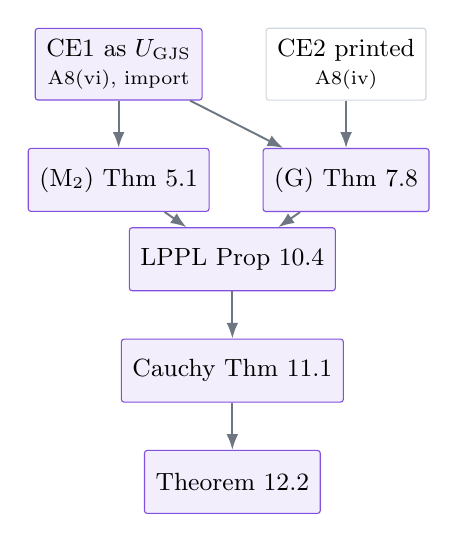
\begin{tikzpicture}[node distance=6mm and 8mm,
  box/.style={draw=gline,rounded corners=1pt,fill=white,align=center,font=\small,
              inner sep=4pt,minimum height=8mm},
  cbox/.style={box,draw=cond,fill=cfill},
  arr/.style={-{Latex[length=2mm]},line width=0.7pt,draw=mut}]
\node[cbox] (ce1) {CE1 as $\UGJS$\\[-1pt]{\scriptsize A8(vi), import}};
\node[box,right=of ce1] (ce2) {CE2 printed\\[-1pt]{\scriptsize A8(iv)}};
\node[cbox,below=of ce1] (m2) {(M$_2$) Thm 5.1};
\node[cbox,below=of ce2] (g) {(G) Thm 7.8};
\node[cbox,below=of $(m2)!0.5!(g)$] (lppl) {LPPL Prop 10.4};
\node[cbox,below=of lppl] (cauchy) {Cauchy Thm 11.1};
\node[cbox,below=of cauchy] (main) {Theorem 12.2};
\draw[arr] (ce1) -- (m2); \draw[arr] (ce2) -- (g); \draw[arr] (ce1) -- (g);
\draw[arr] (m2) -- (lppl); \draw[arr] (g) -- (lppl);
\draw[arr] (lppl) -- (cauchy); \draw[arr] (cauchy) -- (main);
\end{tikzpicture}
\caption{Scaffold test of the F1 spine (final design pending the council).
Violet: conditional on $\UGJS$. Illustration, not evidence.}
\end{figure}

\begin{figure}[ht]
\centering
\begin{tikzpicture}
\begin{loglogaxis}[companion,xlabel={$t$},ylabel={$|W_\gamma(t)|$},
  xmin=1,xmax=160,ymin=1e-8,ymax=1,title={\small filter kernel, $\gamma=1$}]
\addplot[acc!50!white,line width=0.5pt] table[x=t,y=absW]{figures/filter_g1.dat};
\addplot[acc,line width=1.1pt] table[x=t,y=absW]{figures/filter_env_g1.dat};
\end{loglogaxis}
\end{tikzpicture}\hfill
\begin{tikzpicture}
\begin{semilogyaxis}[companion,xlabel={$d$},ylabel={summands of $\Psi_\gamma(d)$},
  xmin=0,xmax=60,ymin=1e-5,ymax=1e3,title={\small rate function, $\gamma=M=1$},
  legend pos=south west]
\addplot[warn,dashed] table[x=d,y=exp]{figures/psi_g1.dat};
\addlegendentry{exponential part}
\addplot[acc] table[x=d,y=tail]{figures/psi_g1.dat};
\addlegendentry{filter tail}
\end{semilogyaxis}
\end{tikzpicture}
\caption{Scaffold test of the computed curves (F3 right, F6), from
\texttt{figures/*.dat}, themselves from \texttt{docs/figures/curves.json}.
One admissible $\chi$; $\Psi_\gamma$ is an upper bound, not a measured decay.
Illustration, not evidence.}
\end{figure}

\begin{checkpoint}
Test of the checkpoint box: $\|(\omega_g-\omega_{g'})|_{\A(O)}\|\le\Psi_\gamma(d)$ whenever
$g\equiv g'\equiv1$ on $O_d$ \rec{Lemma~10.5}{28}.
\end{checkpoint}

\begin{recordbox}{Theorem 12.2 of the record (p.\,30), item (1)}
For every bounded open interval $O$, $\lim_{g\in\G}\|(\omega_g-\omega_\infty)|_{\A(O)}\|=0$.
\end{recordbox}

\begin{context}
Test of the context environment.
\end{context}

\begin{thebibliography}{9}\small
\bibitem{record}\hypertarget{bib-record}{}A.~Stottmeister, \emph{Removal of the spatial cutoff for weakly coupled $P(\varphi)_2$: norm convergence of the ground-state net on the quasi-local algebra, Part~I}, document of record \texttt{part\_i/main.pdf}, 40~pp., version of 5~September 2026, \url{https://github.com/alexander-stottmeister/pphi2-cutoff-removal}.
\end{thebibliography}
\end{document}
